\chapter{Example Showcase}
\label{ch:example}

In this chapter, we seek to demonstrate CheMFC's capabilities beyond the validation
test cases presented in \autoref{ch:validation} by studying the structure
of two-dimensional detonations. As previously described by Kailasanath et al.
\cite{KAILASANATH1985199} and Lefebvre et al. \cite{LEFEBVRE1993206}, this can
be done by simulating a reacting shock tube whose flow upstream of the reaction
front is perturbed to allow for the formation of transverse waves.

To this end, we use results from our one-dimensional reactive shock tube simulation
(\autoref{sec:1d_reactive_shocktube}) to initialize a two-dimensional simulation.
More specifically, we extract the one-dimensional state of the reactive shock tube
once a unique detonation front has formed and reached the Chapman-Jouguet (CJ) velocity.
The two-dimensional initial condition is then constructed by replicating this state
in the $y$-direction, and perturbing the flow upstream of the detonation front with
three rectangular regions of unburned fuel at pressures $1.6$ times greater than that
of the background. In this problem, the left boundary is reflective, the right boundary
is extrapolative, and the top and bottom boundaries are periodic.

The $12$ \si{\centi\meter} $\times$ $6$ \si{\centi\meter} domain is discretized
with $800 \times 200$ grid cells and simulated using the HLLC Riemann solver on
$4$ NVIDIA A100 GPUs and Cantera's \verb|h2o2.yaml| mechanism, a (modified) subset of GRI-Mech 3.0 \cite{GRI30}. A plot
of the numerical schlieren of the results
is shown in \autoref{fig:showcase}, revealing detonation cells similar to those
of Kailasanath et al. \cite{KAILASANATH1985199}.

\begin{figure*}
    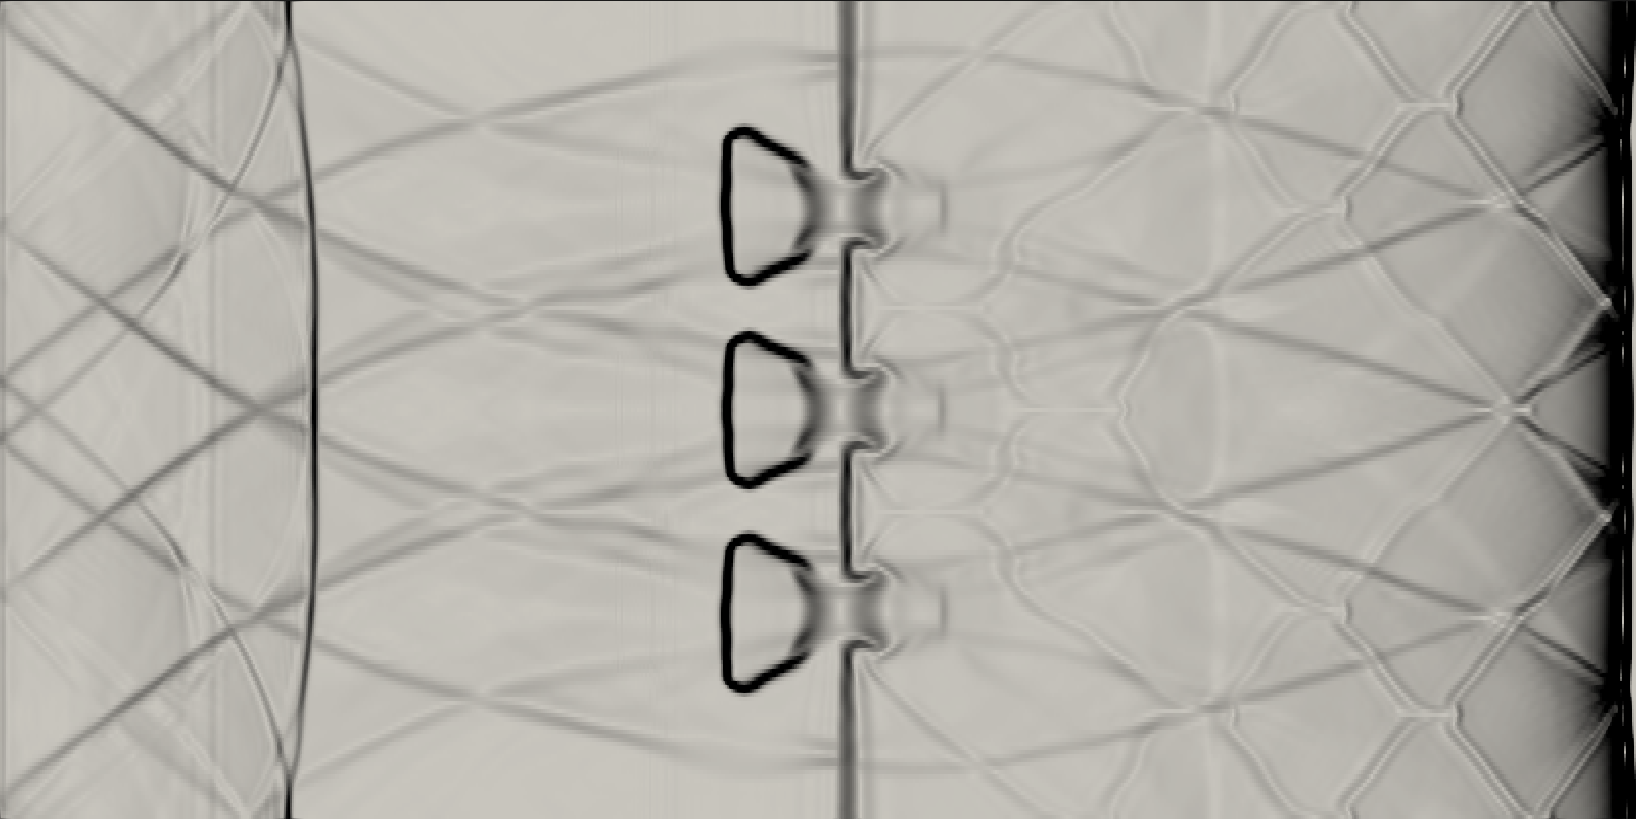
\includegraphics[width=\textwidth]{figures/showcase/simulation.png}
    \caption{Example Showcase: Numerical schlieren of a reacting shock tube whose flow upstream of the reaction
    front is perturbed to allow for the formation of transverse waves. Detonation cells are visible.}\label{fig:showcase}
\end{figure*}